\chapter{Theory}

\section{Objectives, formulation and models}
In order to provide the functionality needed, each of the tools tackles one specific phase. As opposed to a typical analysis workflow, the main objective is maximizing the final user's productivity. Their design therefore hides any numerical complexity, and allows their operation using machine and experimental parameters. Several models are provided as a black-box, which is previously validated by analyst experts, but its source code can be inspected, audited, and extended at any time.

The formulation used for this first implementation is based on the thermal equilibrium using the Principle of Virtual Power. The contributions to the power virtual variation, $\delta \dot \Pi$, are calculated from the numerical integration of the following residual equation:

\begin{equation}\label{eq:var_trabajo}
\delta \dot \Pi = \delta \dot \Pi_{capacitance} - \delta \dot \Pi_{external} - \delta \dot \Pi_{conduction} = 0
\end{equation}

Each of the previous contribution terms can be expressed in the reference configuration \cite{Iglesias2015} as:
\begin{eqnarray}
\label{eq:var_potential_th_internal}
\delta \dot \Pi_{capacitance} & = & \int_{\mathcal B} \rho c_p \frac{dT}{dt} \delta T \ dV
\\
\label{eq:var_potential_th_int}
\delta \dot \Pi_{external} & = & \int_{\mathcal \partial B} \bs q \delta T \cdot \bs n \ dS
\\
\label{eq:var_potential_th_conduction}
\delta \dot \Pi_{conduction} & = & \int_{\mathcal B} \left( \bs \kappa \nabla T \right) \cdot \nabla \delta T \ dV
\end{eqnarray}
Where the conductivity tensor $\bs \kappa$ and the specific heat capacity $c_p$, are temperature dependent, $f(T)$, properties of the material. The density $\rho$ is considered constant.


\begin{figure}[htb]
	\centering
	%  \vspace{-15mm}
	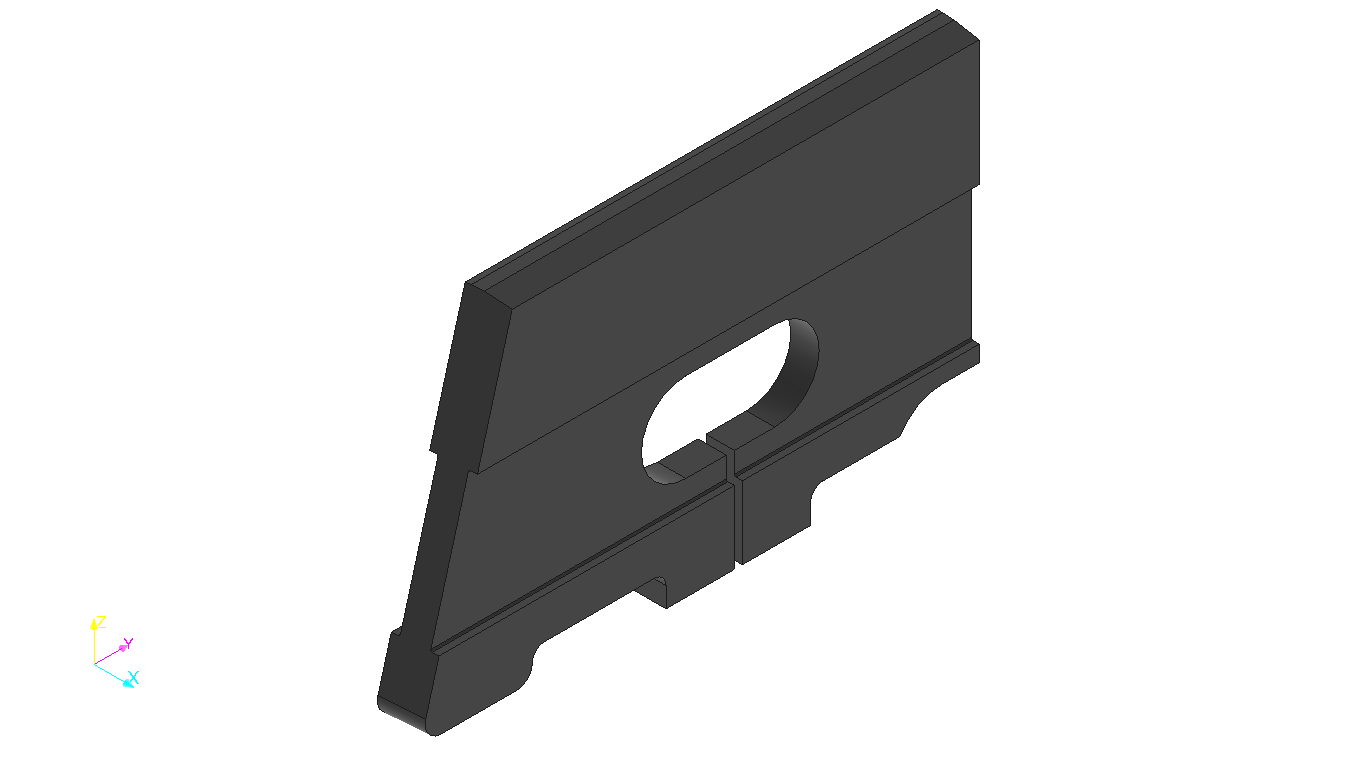
\includegraphics[width=0.48\linewidth,trim={2cm 0 6cm 0},clip]{images/lamella3D-inverse}
	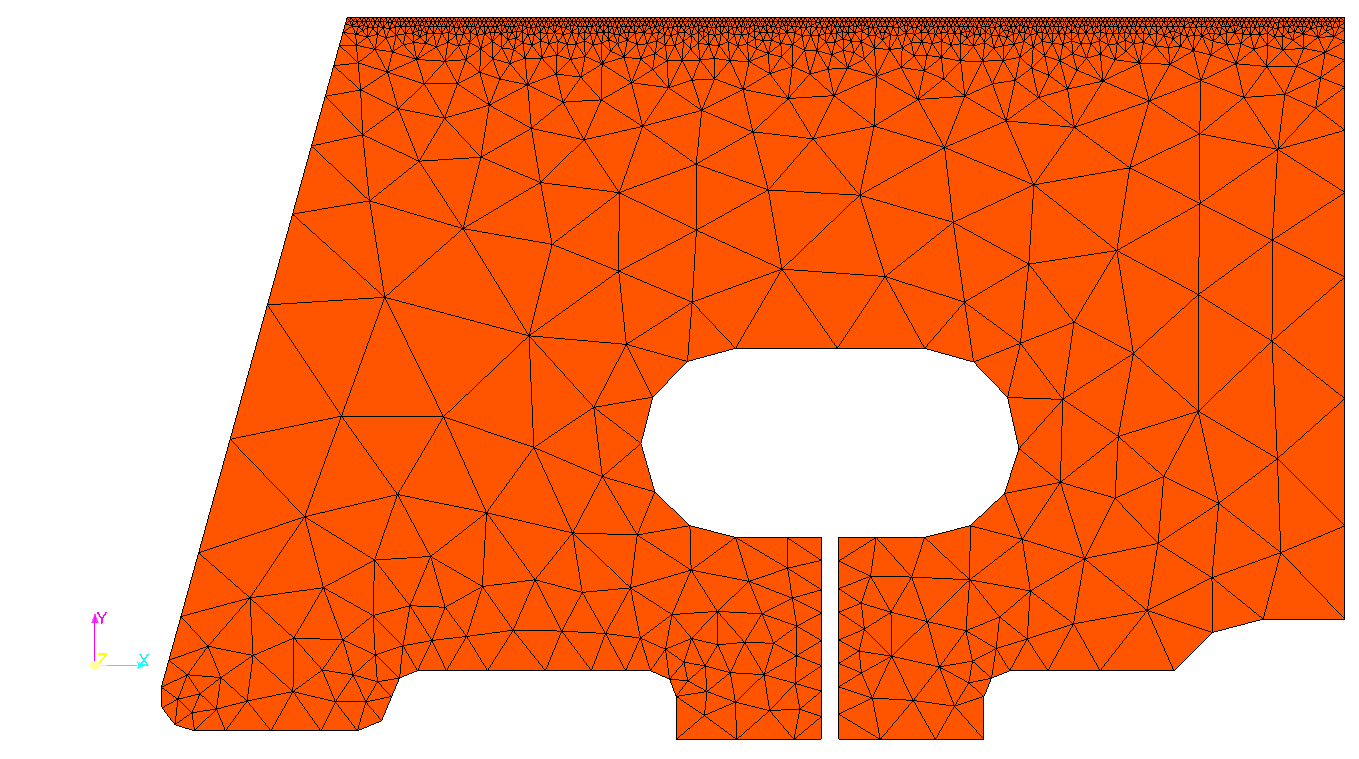
\includegraphics[width=0.40\linewidth]{images/lamella-mesh-inverse}
	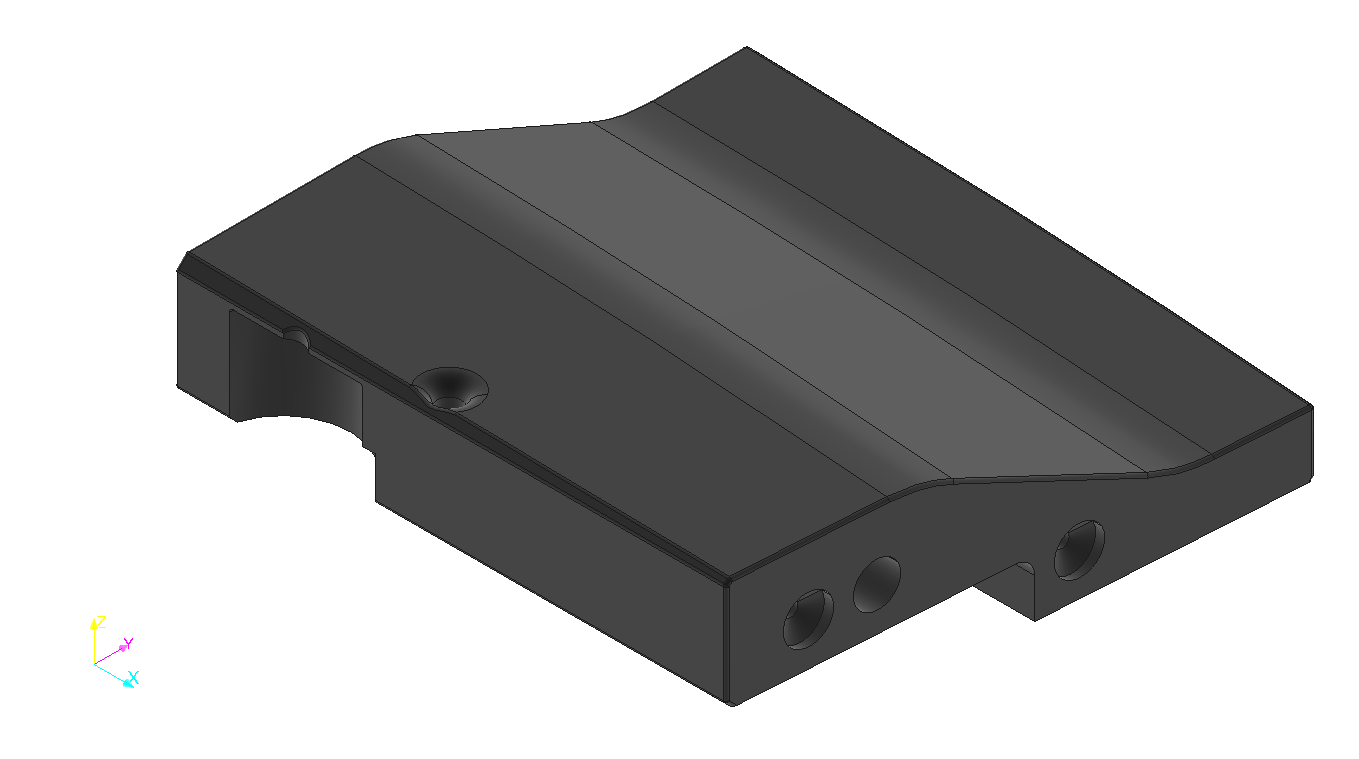
\includegraphics[width=0.50\linewidth]{images/Tile63D-inverse}
	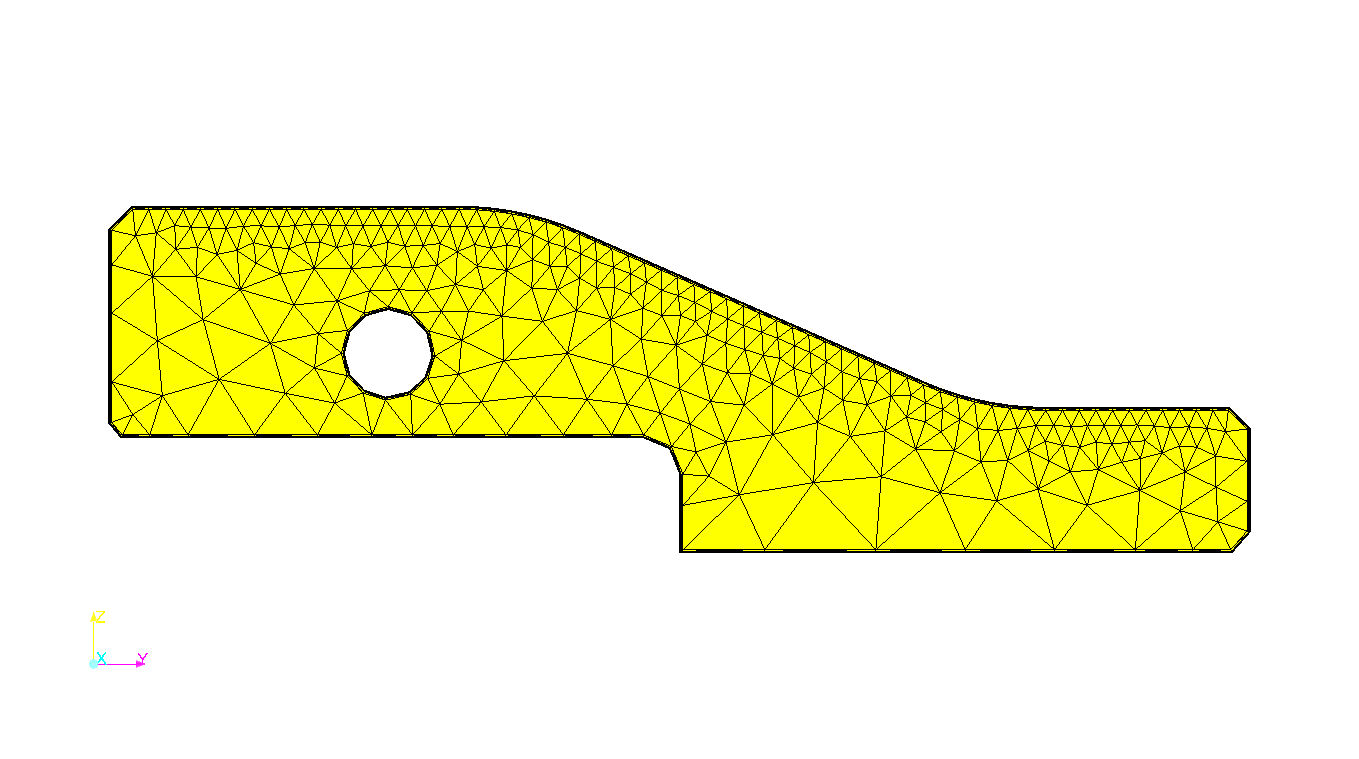
\includegraphics[width=0.48\linewidth]{images/Tile6-mesh-inverse}
	\caption{3D CAD (left) and 2D numerical discretization (right) of divertor components: Tile 5 (top) and tile 6 (bottom).}
	\label{fig:models}
\end{figure}

Fully nonlinear Finite Element (FE) approximations are used for all analyses, with some Galerkin meshfree enhancements \cite{Iglesias2013} when applicable. Several de-featuring levels are applied when speed is a concern. Initial implementation uses 2D models shown in Figure \ref{fig:models}, but design is extensible to 3D in the future. Orthotropic effects, as well as Planck radiation or convection cooling are also foreseen.

Coatings and deposits can be modelled with exact properties, by means of a proper layer formulation which is available for all the applications. Usual parameters for the JET divertor tiles range from 10--\SI{20}{\micro\meter} thickness for the W coating on CFC tiles, to \SI{50}{\micro\meter} node separation in direction normal to the surface for modelling ELMs accurately in bulk W tiles.

